\chapter{Neural Network Fundations}
\section{Basic single layer networks}

\subsection{Linear Layer}
It is known as 'fully connected'/ 'dense' layers

\begin{align}
	y=\sum_{i}w_ix_i+b
\end{align}

	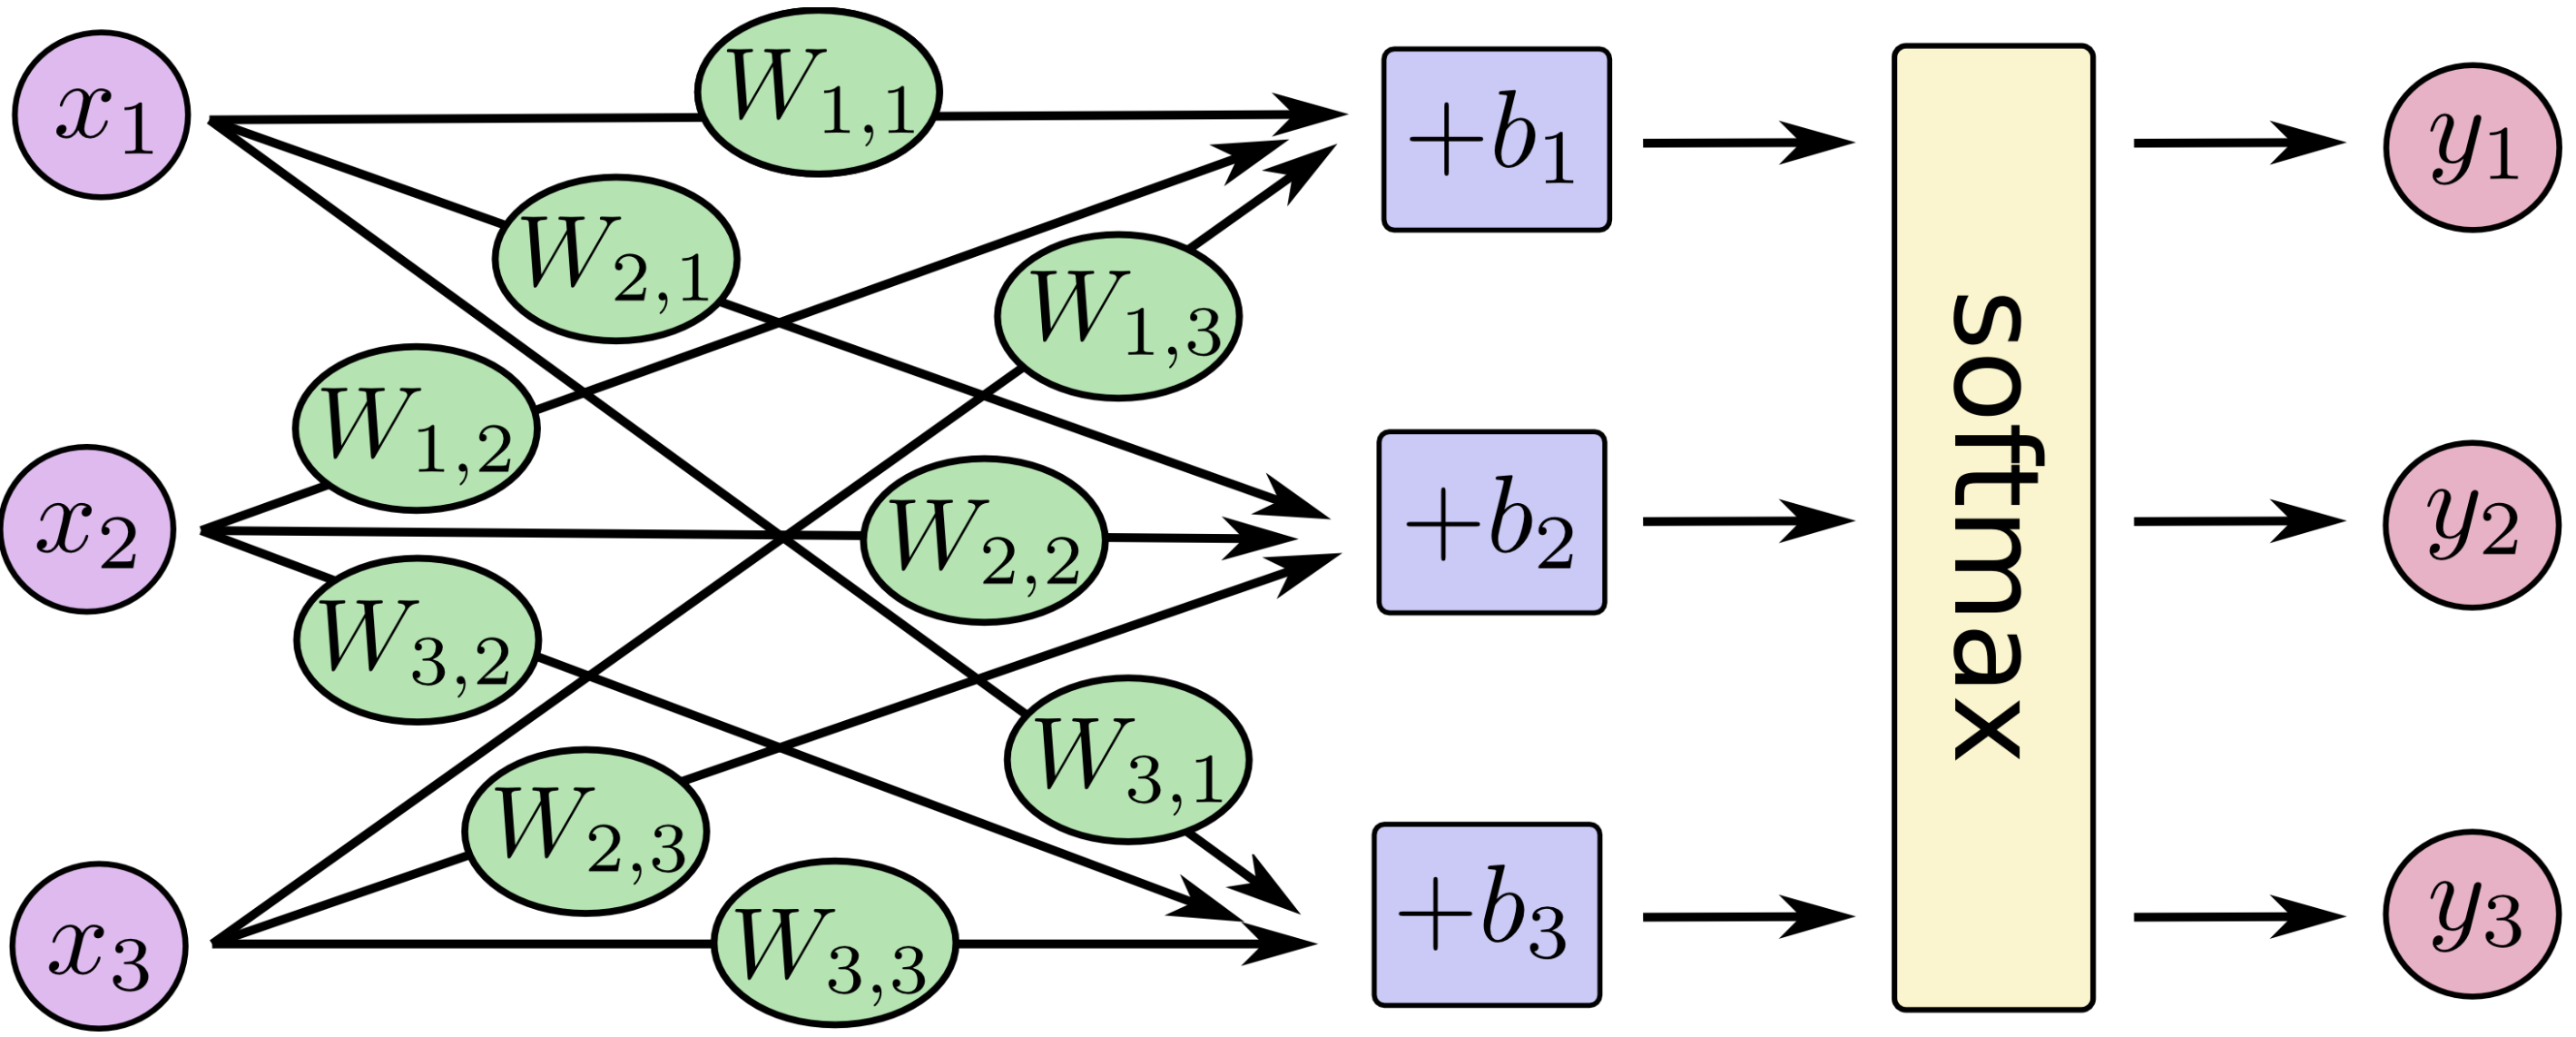
\includegraphics[width=0.4\textwidth]{figures/linear01}

\begin{align}
	\textbf{y}= \textbf{W x} + \textbf{b}
\end{align}	


	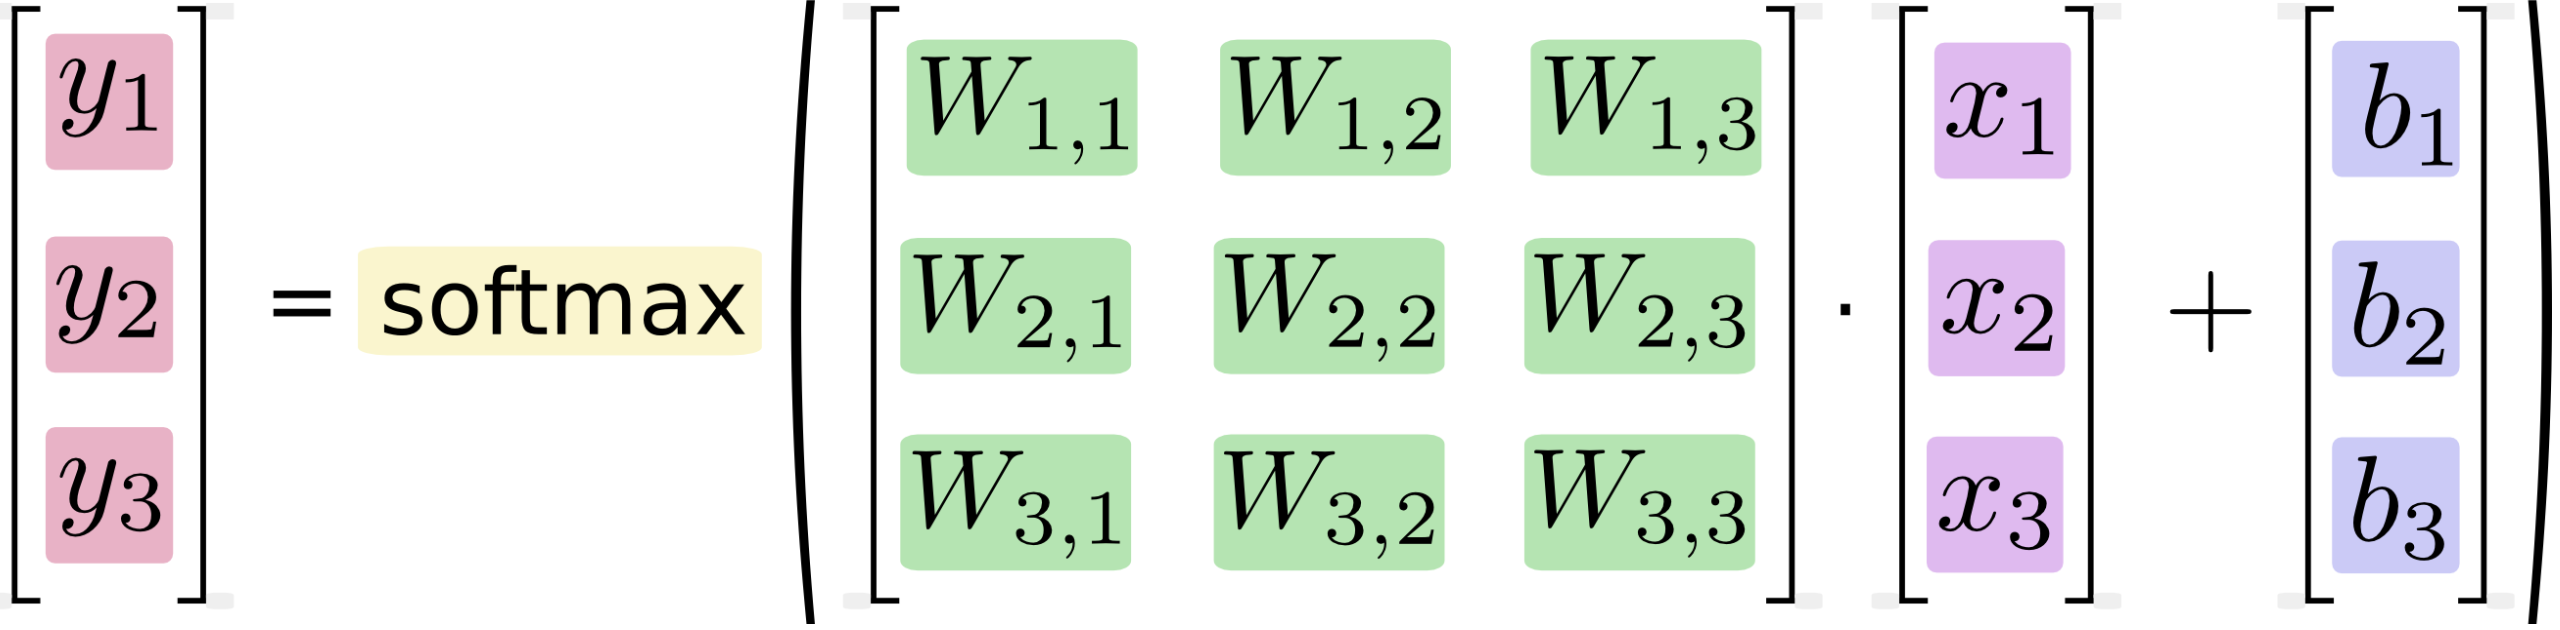
\includegraphics[width=0.4\textwidth]{figures/linear02}

\subsection{Sigmoid Layer}
Sigmoid layer can be used as binary-class classifier with 2-way gating.\\
\textbf{Activation function:} \footnote{For more activation functions see:\\ {\small\url{https://en.wikipedia.org/wiki/Activation_function}}}

\begin{align}
	\sigma(x)=\frac{1}{1+ e^{-x}} = \frac{e^x}{1+e^{x}}
\end{align}

\vspace{-10pt}
\begin{center}
	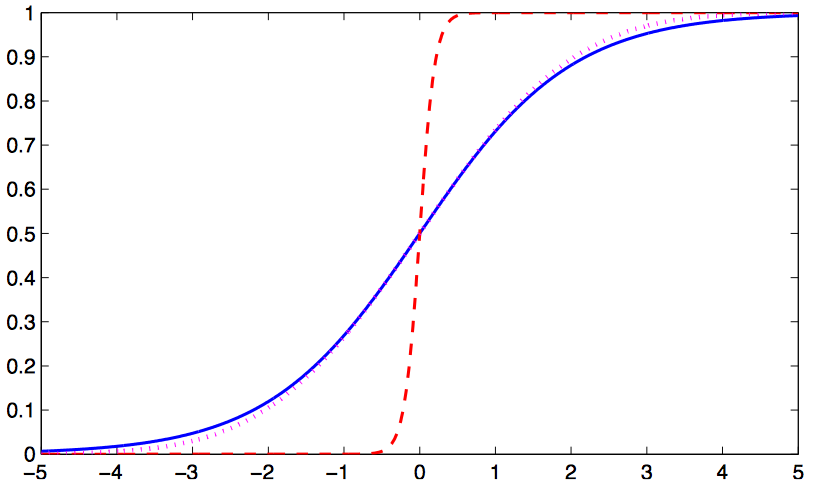
\includegraphics[width=0.4\textwidth]{figures/Sigmoid}
\end{center}


The logistic sigmoid function $\sigma_\beta=1/1+e^{-\beta x} $. The parameter $ \beta $ determines the steepness of the sigmoid. The full (blue) line is for $ \beta=1 $ and the dashed (red) for $ \beta=10 $. As $ \beta \rightarrow \infty $, the logistic sigmoid tends to a Heaviside step function. \\


\textbf{Linear Layer + Sigmoid Layer as a \underline{binary classifier}\\ (Logistirc Regression):}

\begin{align}
	y = f(x) = \sigma(y(x)) = \frac{1}{1+e^{-y}}= \frac{1}{1+e^{-(Wx+b)}}
\end{align}

\begin{center}
	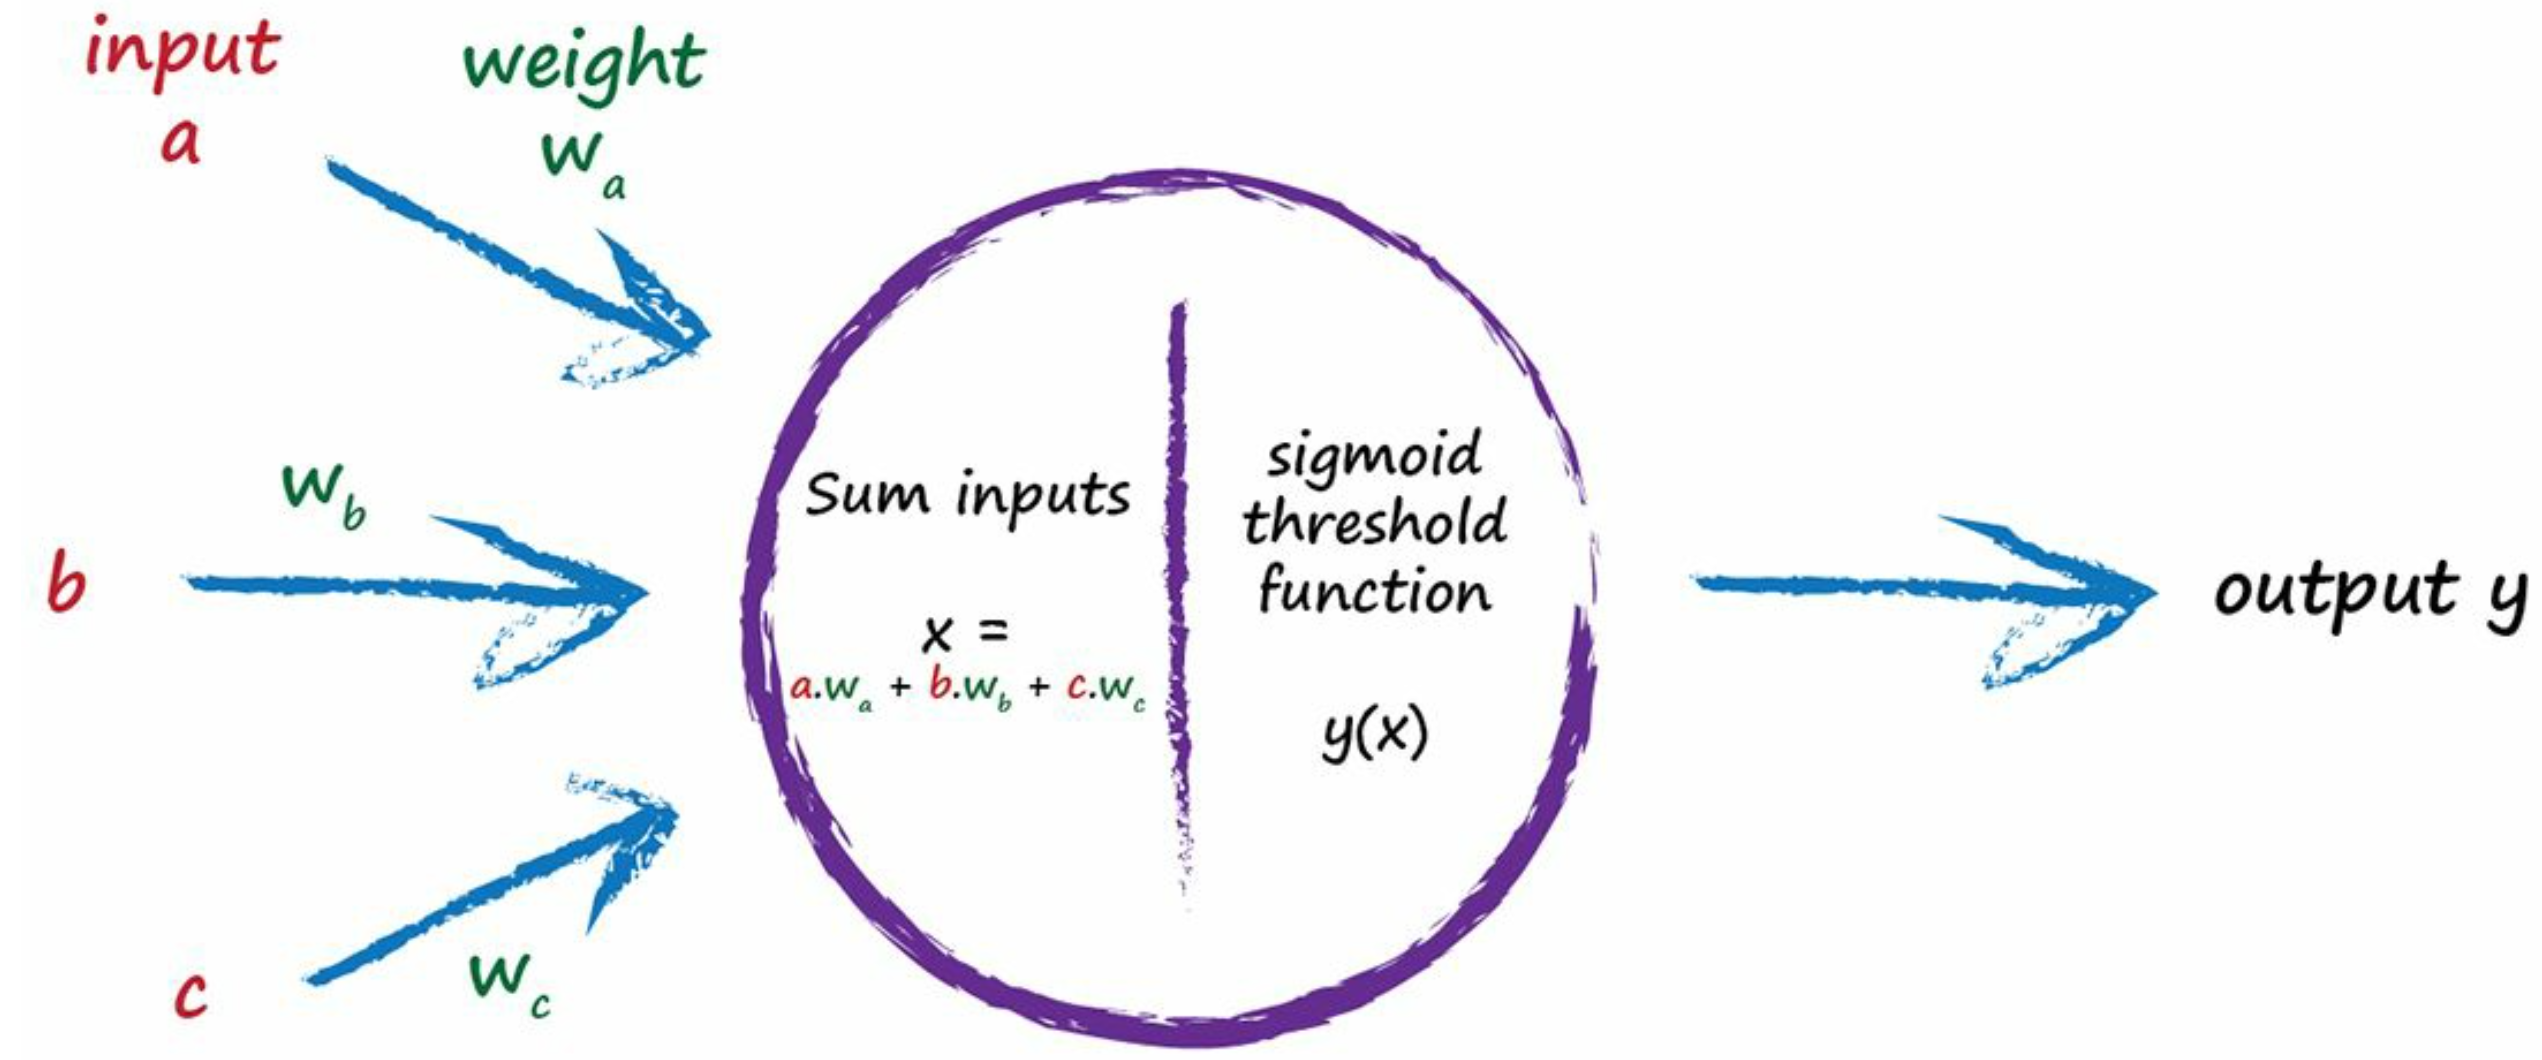
\includegraphics[width=0.55\textwidth]{figures/sigmoid02}
\end{center} 

\textbf{*An alternative activation function is $ \textbf{tanh(x)} $ function:}\\
\vspace{5 pt}
Where $ tanh(x=)f(z) $ here:
\begin{align}
tanh(x)=\frac{e^x-e^{-x}}{e^x+e^{-x}}
\end{align}
\vspace{10pt}
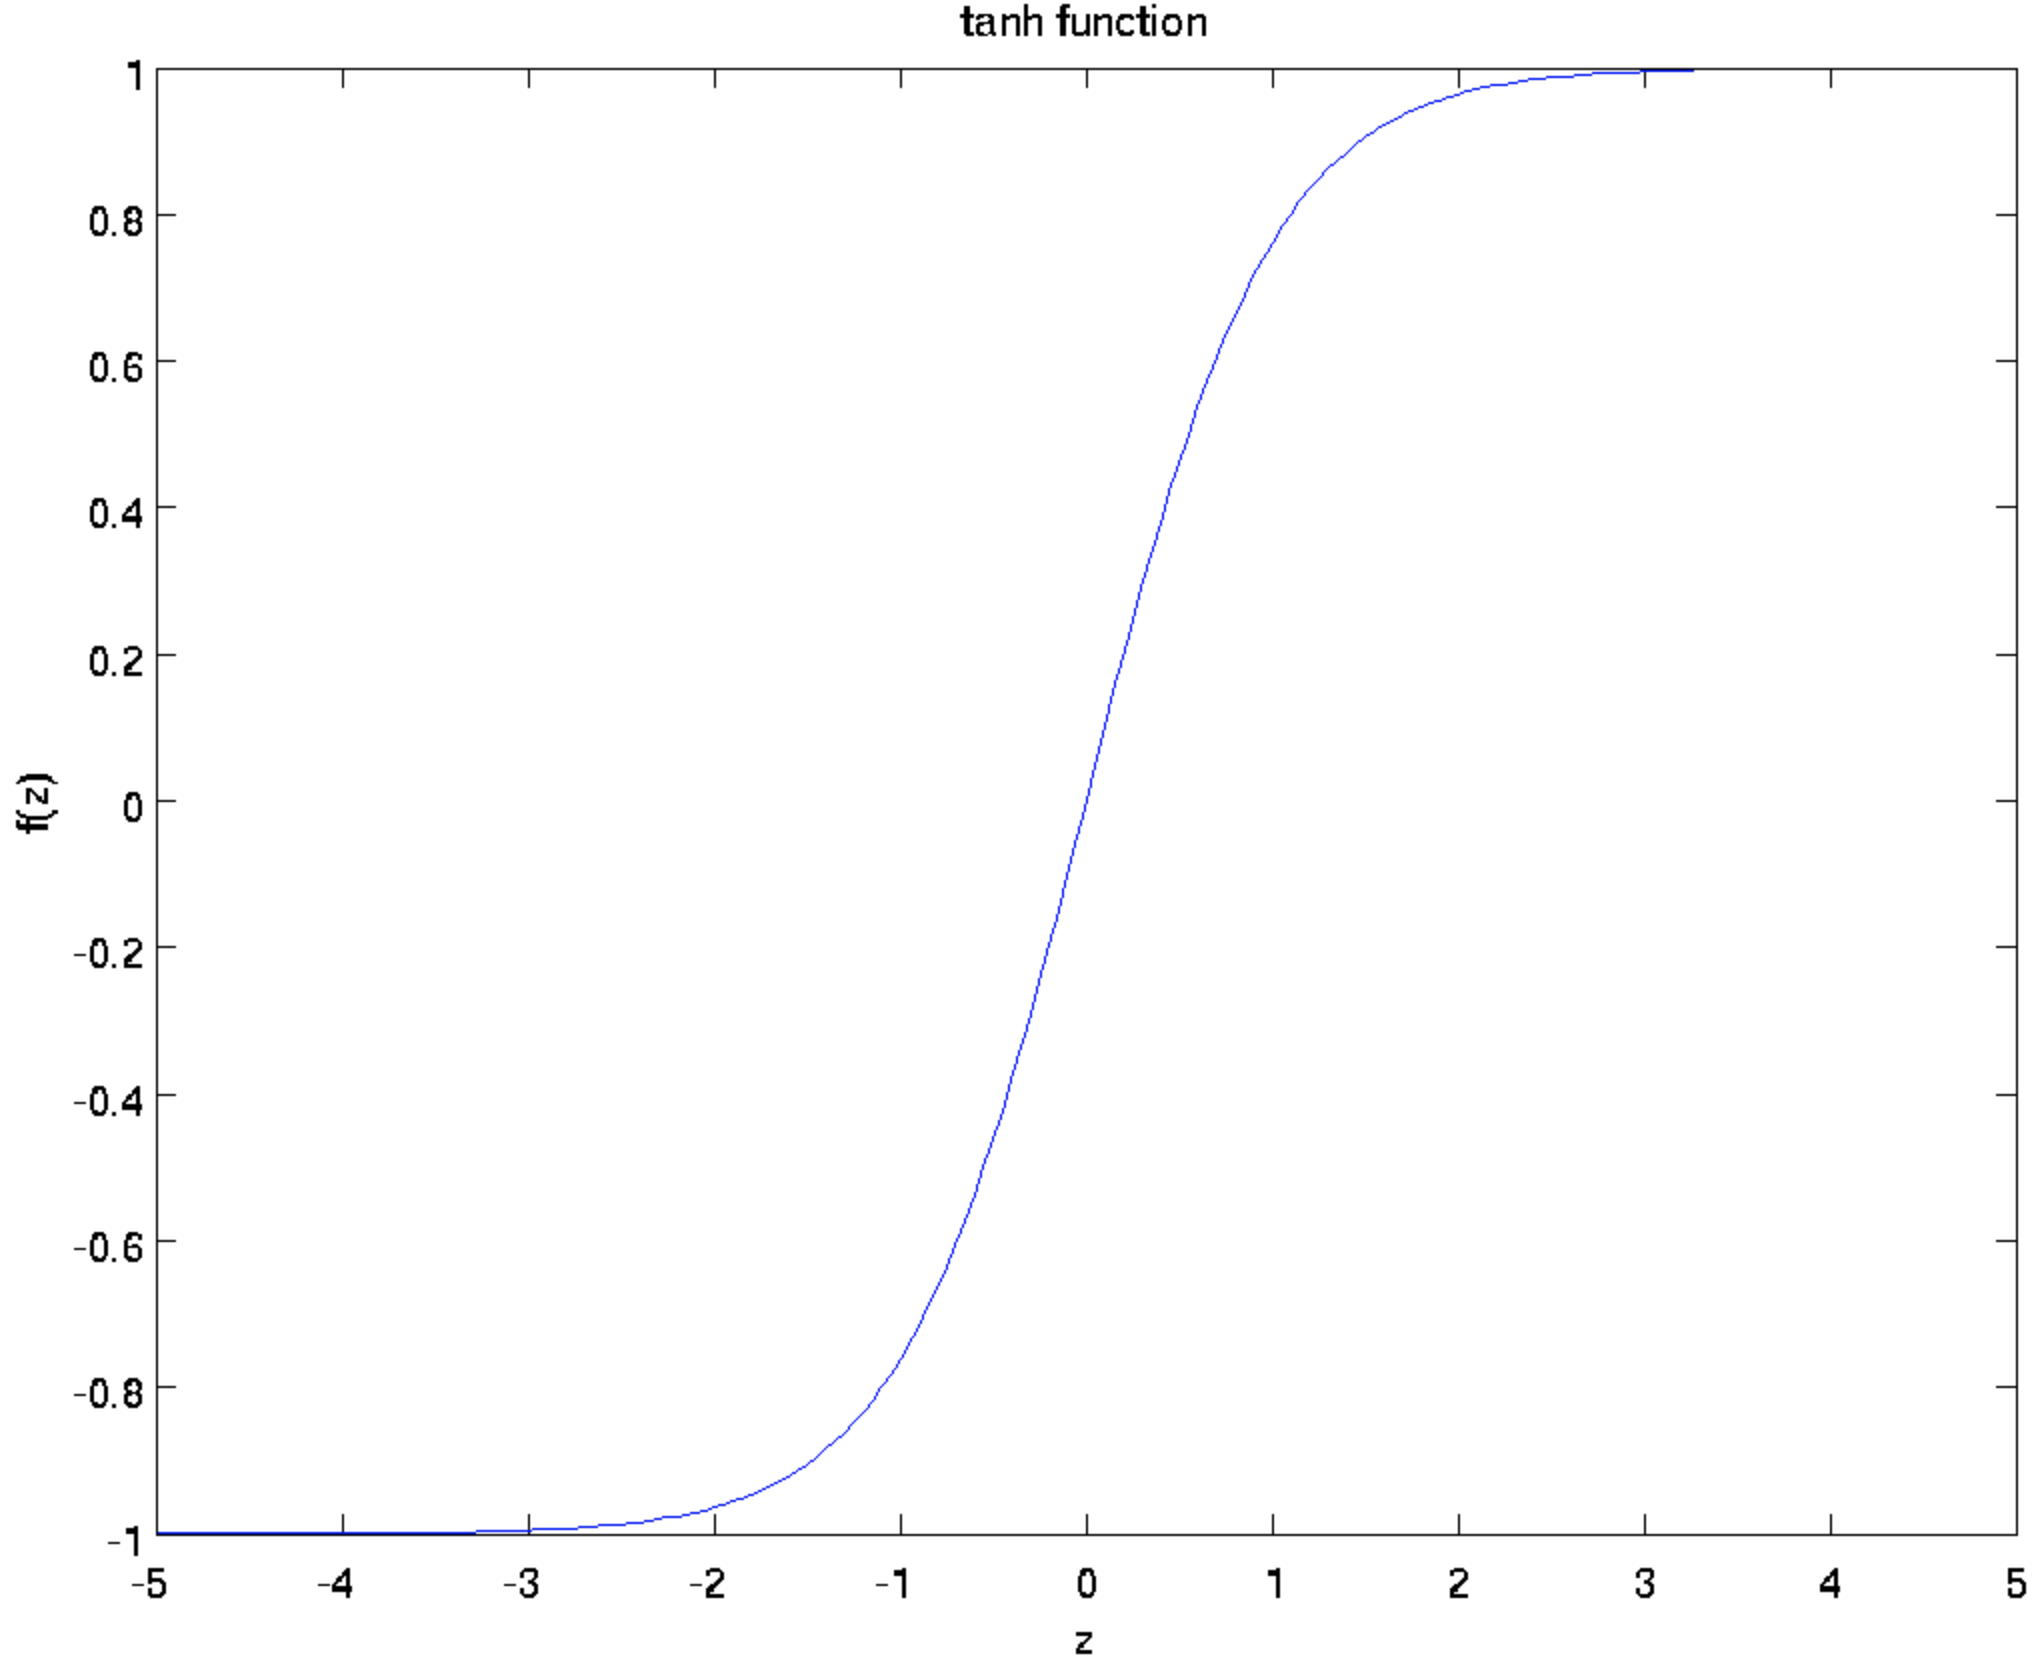
\includegraphics[width=0.55\textwidth]{figures/tanh}

\subsection{Softmax Layer}
Softmax layer can be used as multi-class classification and also in soft/differentiably multi-way gating/routing.

\begin{flalign}
	&&y &= softmax(x)&\\
	&\text{with, }&y_i &=\dfrac{e^{x_i}}{\sum_{j=1}^{K}e^{x_j}}&
\end{flalign}


\textbf{LinearLayer + SoftmaxLayer as a \underline{multi-class classifier}:}\\

\vspace{-10pt}

\begin{align}
	 y_i=\dfrac{e^{\sum_{j}w_{ij}x_i+b_i}}{\sum_{k}e^{\sum_{j}w_{kj}x_j+b_k}} 
\end{align}


\subsection{Rectified-linear Layer (ReLU)}
ReLU is simpler/ cheaper than sigmoid, and it is prevalent in modern neural nets.
\begin{flalign}
	&&y&=ReLU(x) &\\ 
	&\text{with, }&y_i &=max(0, x_i)&
\end{flalign}
%\vspace{-10pt}
\begin{center}
		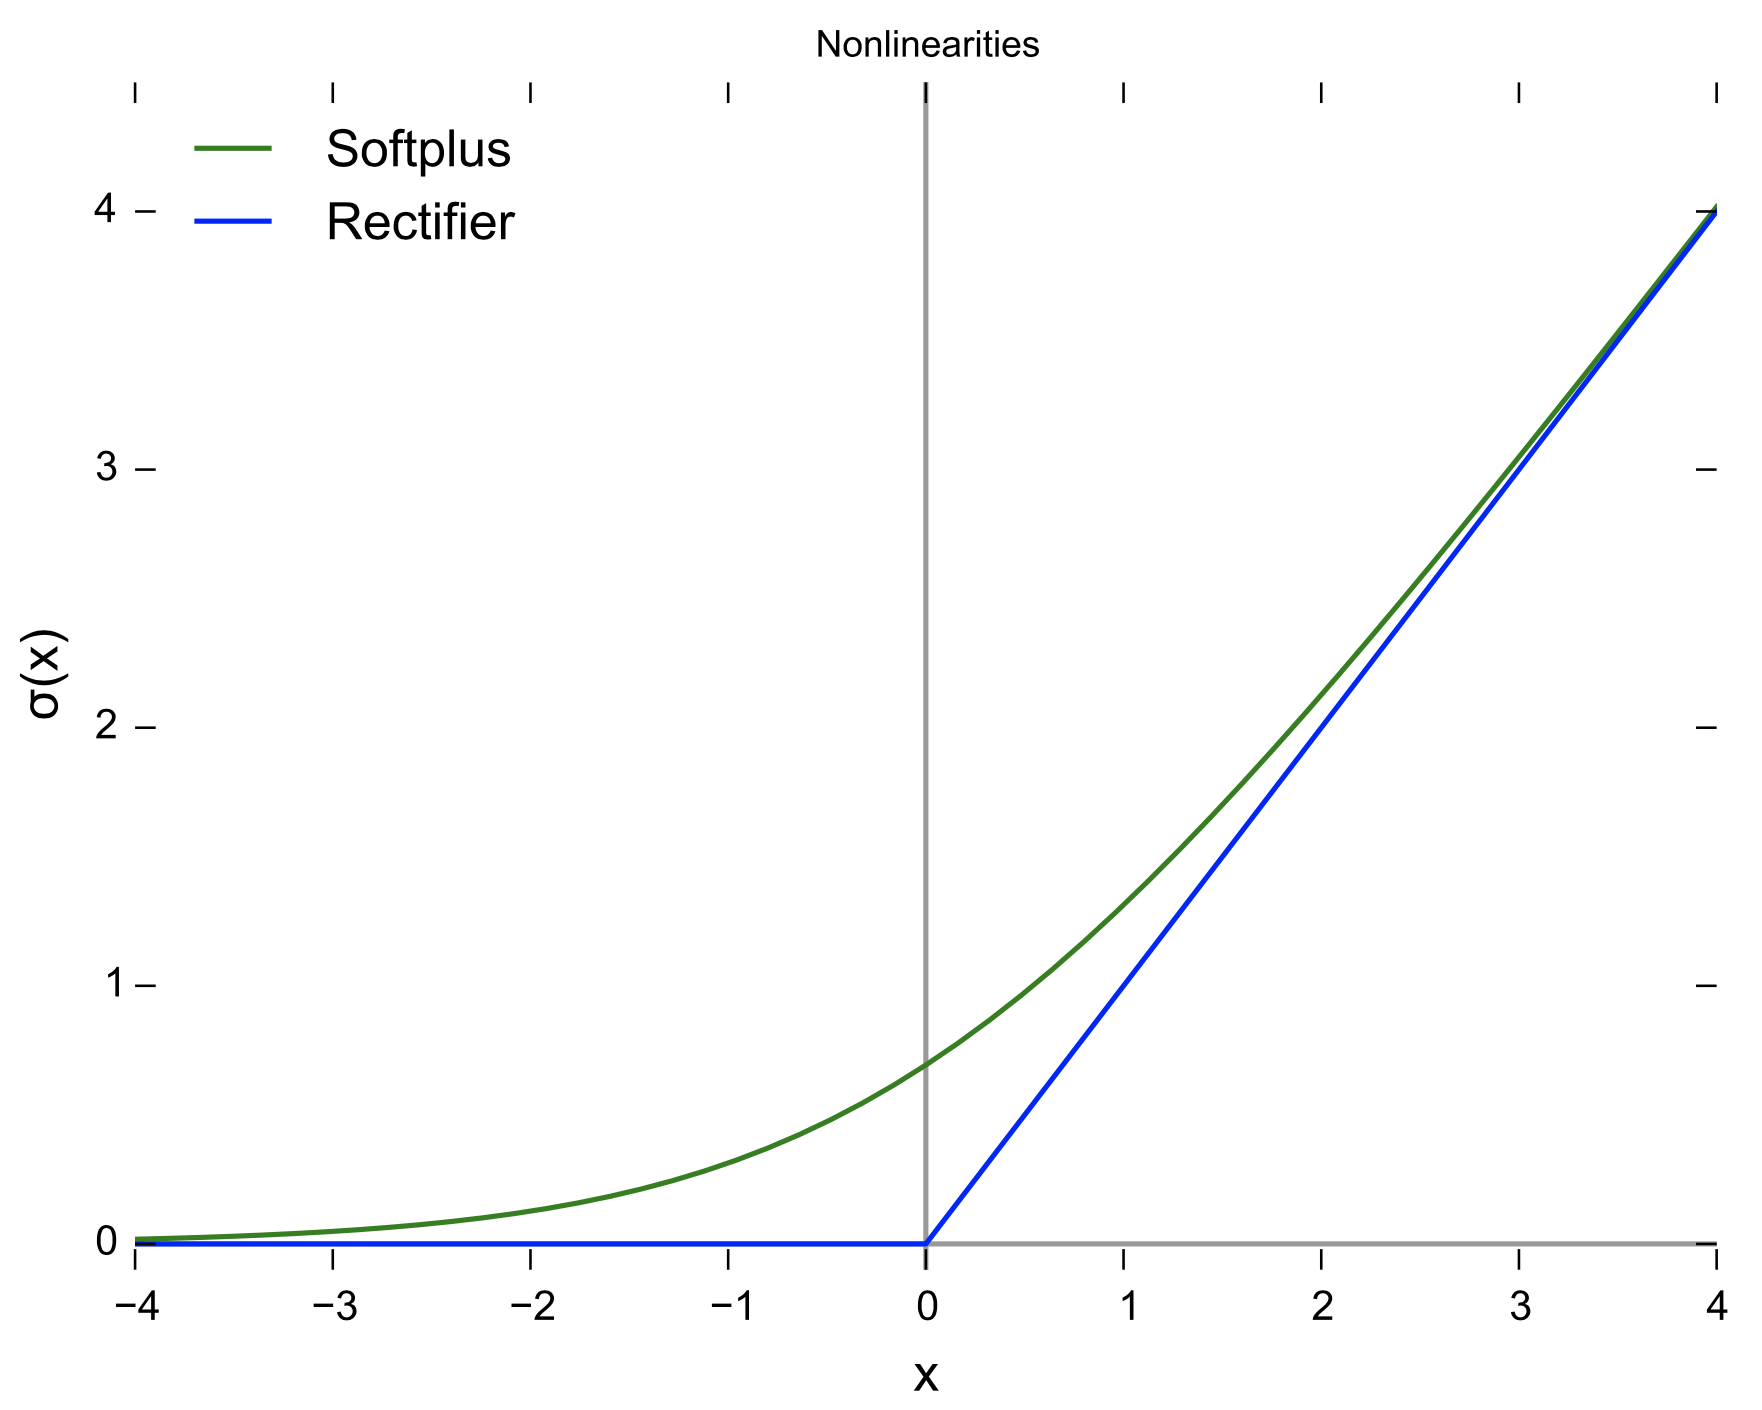
\includegraphics[width=0.35\textwidth]{figures/ReLU}
\end{center}




